\documentclass[a4paper, 11pt]{article}
\usepackage[top=2cm, bottom=2cm, left = 2cm, right = 2cm]{geometry} 
\geometry{a4paper} 

\usepackage[T1]{fontenc}
\usepackage[utf8]{inputenc}
\usepackage{lmodern}
\usepackage[ngerman]{babel}
\usepackage{microtype}


\usepackage{graphicx} 
\usepackage{amsmath,amssymb}  
\usepackage{bm}  
\usepackage[pdftex,bookmarks,hidelinks,breaklinks]{hyperref}  

\title{Praktikumsbericht Audiosignalverarbeitung}
\author{Franko Jolic, Janne Buhr}
%\date{}

\begin{document}
\AddToHook{cmd/section/before}{\clearpage}
\begin{titlepage}
    \maketitle
    \tableofcontents
    \vfill
\end{titlepage}

\section{Aufgabenblatt 1}

    \subsection{Frage 1}
    Wie funktioniert eine Authentifizierung mit SHH-Schlüsseldateien (SSH keys)? Was ist die Grundidee und wie welche Schritte müssen ausgeführt werden?

    \subsection{Frage 2}
    Wofür genau benötigt man eine virtuelle Umgebung? Was sind die Vorteile?

\section{Aufgabenblatt 2}

    \subsection{Kurzvortrag}
    Wird in der Datei vortrag.text weiter ausgeführt

\section{Aufgabenblatt 3}

    
    
    \begin{figure}
    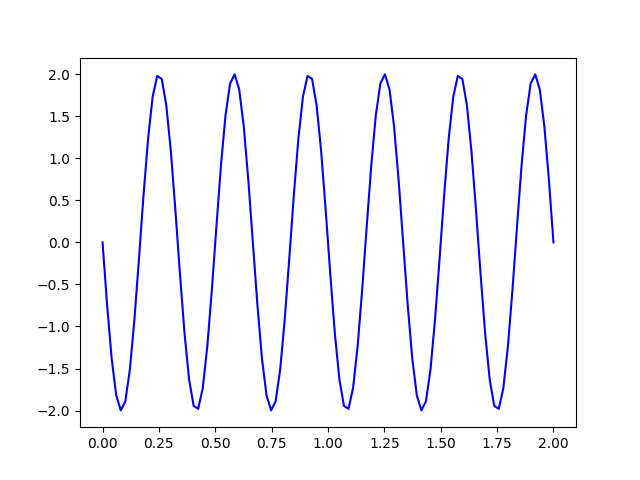
\includegraphics[width =0.5\textwidth]{plot.png}
    \caption{Hier kommt die Bildunterschrift hin.}
    \label{fig : label1}
    % Abbildung kann im Text mit \ ref { fig : label1 }
    % referenziert werden
    \end{figure}


    \subsection{Was ist eine Frequenz?}
    
    \subsubsection{Frage 1}
    Bei akustischen Signalen entscheidet vorallem die Frequenz der Schwingungen über die wahrgenommene Tonhöhe. 
    Welche Frequenzen liegen im hörbaren Bereich\\
    Je nach Alter und individuellen Eigenschaften hören Menschen Frequenzen von 20 bis 20000 Hz.


    Länge voller wiederholung 1 drittel sekunde 

    \subsection{Das Abtasttheorem}
    Notiert eure Vermutungen zu den obigen Fragen an dieser Stelle!
    \subsubsection{Fragen und Antworten zur ersten Teilaufgabe}
    Welche Grundfrequenz hat das periodische Signal? 
    \begin{itemize}
    \item Das periodische Signal hat eine Grundfrequenz von 1Hz.  
    \end{itemize}
    Was sind die Frequenzen der sinus und kosinusförmigen Teilsignale?
    \begin{itemize}
        \item Die Frequenz des sinusförmigen Teils liegt bei 2Hz
        \item Die Frequenz des cosinusförmigen Teils setzt sich zusammen aus 1Hz + 3Hz also 4Hz 
    \end{itemize}
    Ließe sich das kontinuierliche Signal s\textsubscript{a}(t) nur aus den Abtastwerten rekonstruieren? Oder sind informationen verloren gegangen, die dies unmöglich machen?
    \begin{itemize}
        \item Durch die Verringerung der Abtastrate sind wichtige Informationen verloren gegangen, wie beispielsweise der weitere Verlauf der Funktion, sowie Minima und Maxima die nicht mehr deutlich sind 
        also kann man das kontinuierliche signal nicht mehr rekonstruieren.
    \end{itemize}
    Ändert die Abtastrate und schaut euch die entsprechenden Plots an. Welche Rolle könnte die Abtastrate dabei spielen?
    \begin{figure}
        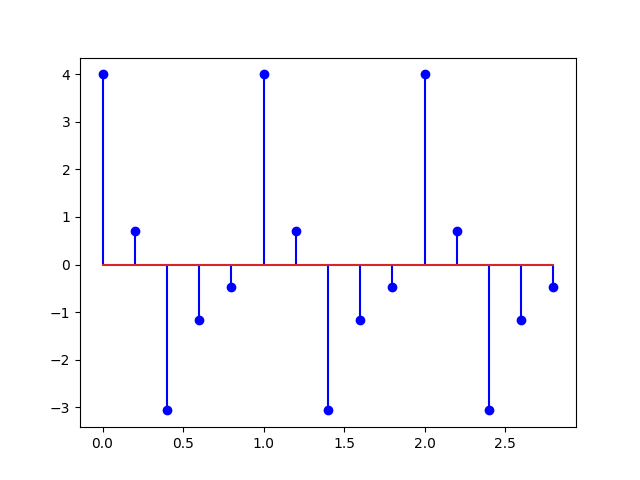
\includegraphics[width =0.5\textwidth]{Abild220.png}
        \caption{Abtastrate von 5}
        \label{fig : label2}
        % Abbildung kann im Text mit \ ref { fig : label1 }
        % referenziert werden
        \end{figure}
    
        \begin{figure}
            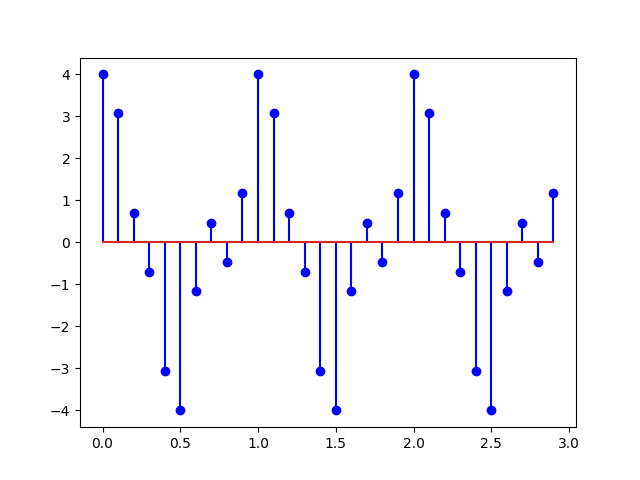
\includegraphics[width =0.5\textwidth]{Abild221.png}
            \caption{Abtastrate von 10}
            \label{fig : label3}
            % Abbildung kann im Text mit \ ref { fig : label1 }
            % referenziert werden
            \end{figure}

            \begin{figure}
                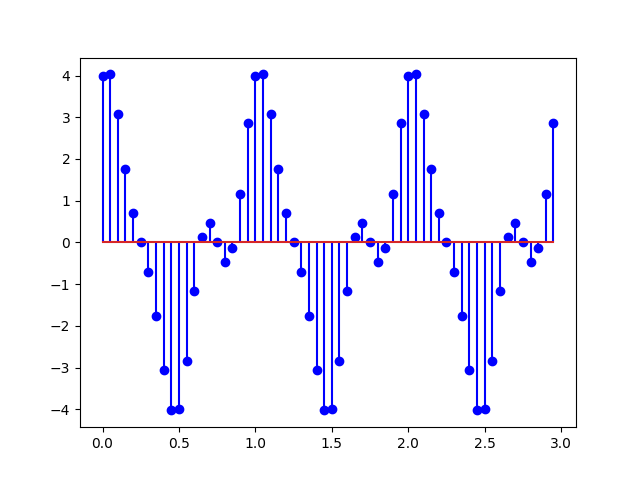
\includegraphics[width =0.5\textwidth]{Abild222.png}
                \caption{Abtastrate von 20}
                \label{fig : label4}
                % Abbildung kann im Text mit \ ref { fig : label1 }
                % referenziert werden
                \end{figure}
    
    
                    \begin{itemize}
                    \item Wie man unten anhand der 3 Abbildungen sieht haben wir die Abtastrate zuerst auf 5 runtergesetzt und danach auf 20 erhöht. 
                    Man erkennt ganz genau das wir desto höher unsere Abtastrate ist, unsere Abbildung immer näher an das Original rankommt.
                    \end{itemize}
    
    
   
    
    \subsubsection{Frage 2}
    
    
    
    


    
    
    \subsection{Frage 4}
     Lässt sich das Originalsignal aus den Abtastwerten rekonstruieren?
     Ist die Rekonstruktion für alle Funktionswerte gleich gut?
     Woran könnte es liegen, wenn ihr hier unterschiede feststellt?
     Was passiert, wenn ihr die Abtastrate verringert oder erhöht?
     Gibt es einen kritischen Wert bei dem eine sich etwas grundsätzlich verändert?
     Beantwortet diese Fragen in eurem Bericht mit Hilfe von passenden Abbildungen. Entsprechen die Ergebnisse euren Vermutungen?


    \subsection{Frage 5}
    Wie verhalten sich die Frequenz des Signals und die Mindestabtastrate zu einander?
    Wie passt eure Beobachtung hier zu den Beobachtungen für das zusammengesetzte Signal s\textsubscript{a}?

    \subsection{Frage 6}
    Das berühmte und wichtige Abtasttheorem formalisiert eure Beobachtungen. Könnt ihr es formulieren?


\section{Aufgabenblatt 4}

\section{Aufgabenblatt 5}

\section{Aufgabenblatt 6}

\section{Aufgabenblatt 7}

\section{Aufgabenblatt 8}

\section{Aufgabenblatt 9}

\section{Aufgabenblatt 10}

\end{document}